\documentclass{article}

\usepackage[T1,T2A]{fontenc}
\usepackage[utf8]{inputenc}
\usepackage[english,russian]{babel}

\usepackage{pdfpages}
\usepackage{multirow}

\usepackage{caption}

\usepackage{amsmath}
\usepackage[hidelinks]{hyperref}


\usepackage{graphicx}%Вставка картинок
\graphicspath{{noiseimages/}}

\usepackage{float}%"Плавающие" картинки
\usepackage{wrapfig}%Обтекание фигур (таблиц, картинок и прочего)

\makeatletter
\def\@biblabel#1{#1. }
\makeatother

\setlength{\emergencystretch}{10pt}

\begin{document}

Попробуем посчитать значения по двум формулам и сравнить полученный результат

Характеристики ванны:

3.5 на 10

аноды: 17.5

МПР: -

t=960



\begin{figure}[H]
\centering
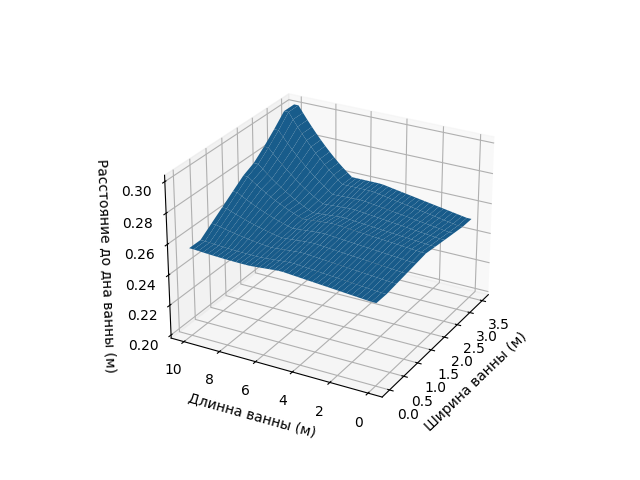
\includegraphics[width=0.8\linewidth]{surf1.png}
\caption[]{}
\label{fig:elec}
\end{figure}

Surf1:

Мин МПР: 80.40417519352799

0.013904088195094139

\begin{figure}[H]
\centering
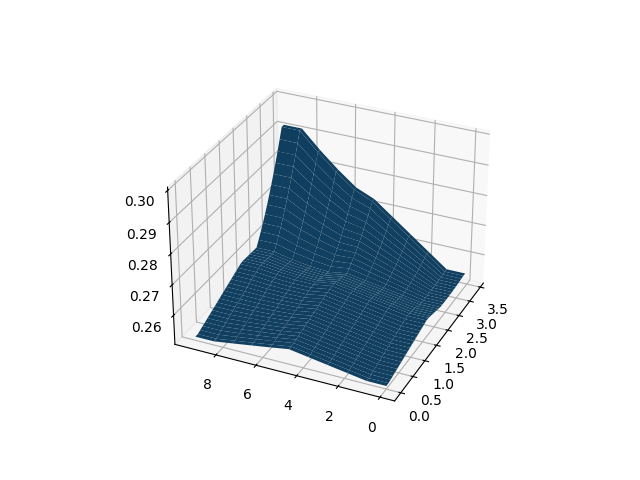
\includegraphics[width=0.8\linewidth]{surf2.png}
\caption[]{}
\label{fig:elec}
\end{figure}

Surf2:

Мин МПР: 86.00298228109142

0.010538644927029358


Для h

87.33771891563774

90.21197903908192

0.016524174090314994

0.016128757090317393


\end{document}